\documentclass{article}

\usepackage{url} 

\usepackage{pdfpages}
\usepackage{lastpage}
\usepackage{fancyhdr}
\usepackage{ngerman}
\usepackage{listings}

\usepackage{floatrow}
\usepackage[tableposition=top]{caption}
\floatsetup[table]{capposition=top}

\usepackage{amsmath, amssymb}

\usepackage[utf8]{inputenc}


\usepackage[numbib]{tocbibind}



\newcommand\twodigits[1]{%
   \ifnum#1<10 0#1\else #1\fi
}



\lhead{Dünne Linsen}
\rhead{9. Oktober 2020\\T. Maier, J. Winkler}
%\cfoot{\twodigits{\thepage}~/ \pageref{LastPage}}
\cfoot{{\thepage}~/ \pageref{LastPage}}

\begin{document}

\parindent0cm

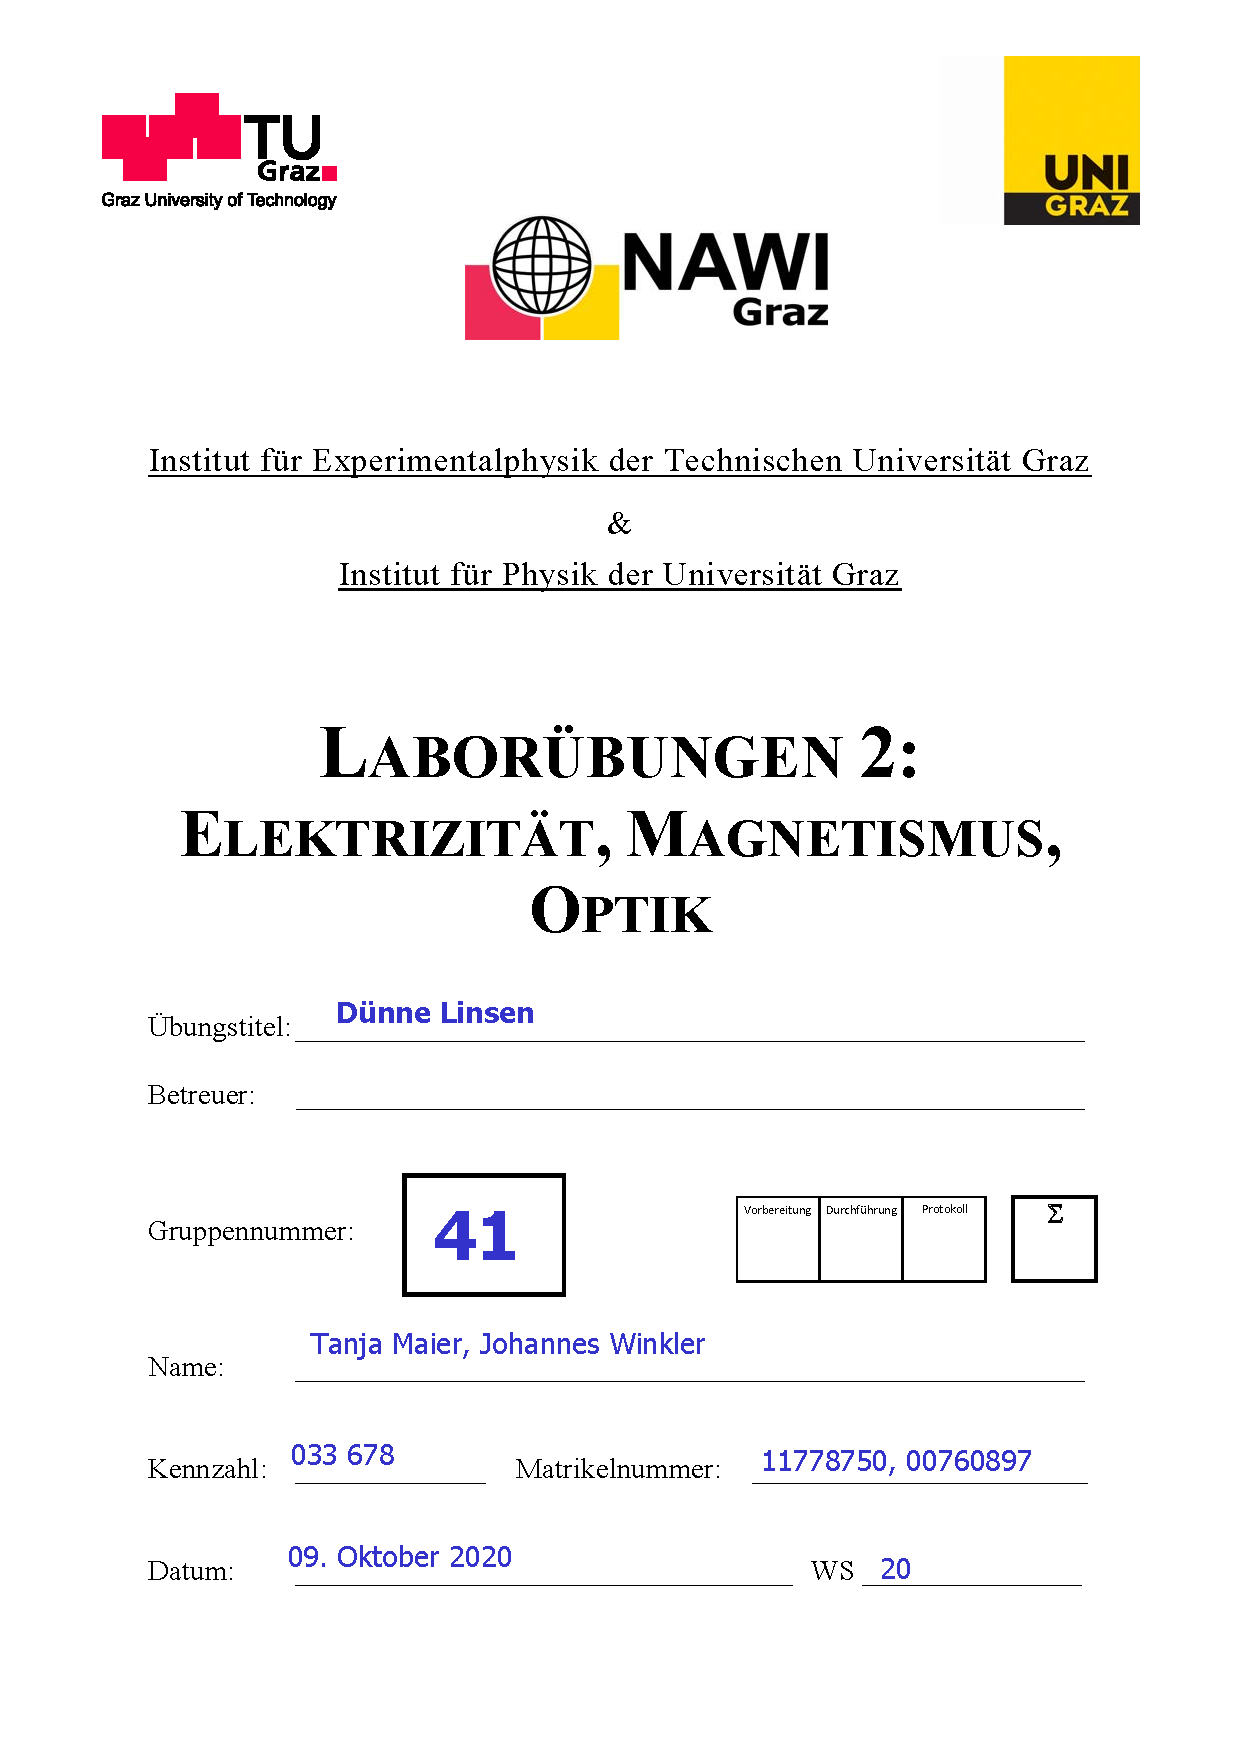
\includepdf{Deckblatt.pdf}


\pagestyle{fancy}

\section{Aufgabenstellung}

\begin{enumerate}
\item Justieren der optischen Anordnung mittels Laser und Lochblende.
\item Die Brennweite einer dünnen Sammellinse ist nach \ref{sec:laplace} 10 mal für verschiedene Gegenstands und Bildweiten zu messen.

Deren Unsicherheiten sind nach Größtunsicherheitsmethode zu bestimmen -- Das endgültige Messergebnis wird statistische ermittelt.
\item Bestimmung der Brennweite durch grafische Auswertung der $b^{-1}$ über $g^{-1}$ Darstellung auf mm-Papier (oder mit einem Programm) gemäß Gleichung \eqref{eq:laplace} mit Angabe der Unsicherheiten $\Delta(g^{-1})$ und $\Delta(b^{-1})$.

\item Für 5 verschiedene Gesamtabstände $a$ (siehe Abb. \ref{fig:bessel}) ist die Brennweite derselben Linse nach dem Bessel'schen Verfahren (Abschnitt \ref{sec:bessel}) zu kontrollieren.

\item Es ist nach Abschnitt \ref{sec:zerstr_methode1} die Brennweite der Zerstreuungslinse 10 mal für verschiedene Gegenstands- und Bildweiten zu messen. Das Messergebnis ist statistisch zu ermitteln.

\item Einige Linsenfehler/Unsicherheitsfaktoren sollten durch geeignetes Experimentieren dargestellt bzw. abgeschätzt werden.
\end{enumerate}


\section{Grundlagen und Versuchsaufbau}

\subsection{Sammellinse}

\subsubsection{Laplace'sche Methode}
\label{sec:laplace}

Durch Messen von $g$ und $b$ bei \textit{scharfer} Abbildung kann die Brennweite $f$ einer dünnen Sammellinse aus der Laplace'schen Abbildungsgleichung bestimmt werden:
\begin{align}\label{eq:laplace}
\frac1f = \frac1g + \frac1b
\end{align}

\begin{figure}[H]
\centering
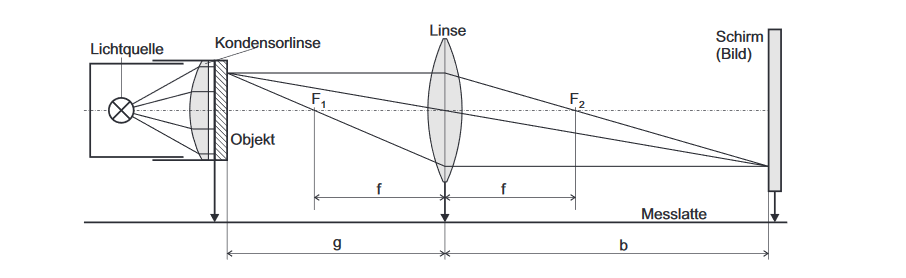
\includegraphics[scale=0.5]{laplace.png}
\caption{Schema des Aufbaues. Bildkonstruktion für einen Objektpunkt nach der geometrischen Optik. $g$ Gegenstandsweite, $b$ Bildweite, $f$ Brennweite, $F_1$, $F_2$ Brennpunkte.}
\label{fig:laplace}
\end{figure}


\subsubsection{Bessel'sches Verfahren}
\label{sec:bessel}

Hier wird der Grundsatz von der Umkehrbarkeit der Lichtwege ausgenützt. Es gelingt unter der Voraussetzung $g+b >4\cdot f$ für zwei Gegenstands- bzw. Bildweiten je eine reelle Abbildung zu erhalten (Abb. \ref{fig:bessel}). Die Brennweite steht mit der dazu notwendigen Verschiebung $e$ und dem Gesamtabstand $g+b=a$ in folgendem Zusammenhang:
\begin{align}
\label{eq:bessel}
f = \frac14 \cdot \left( \frac{a^2-e^2}{a}\right)
\end{align}
\begin{figure}[H]
\centering
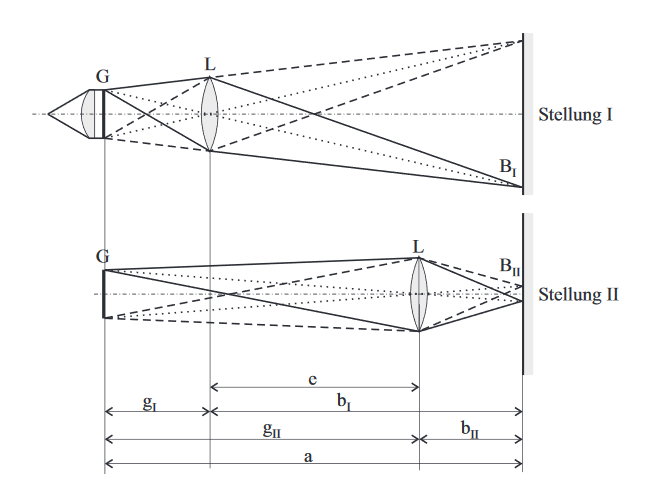
\includegraphics[scale=0.5]{bessel.png}
\caption{Die Bessel'sche Anordnung zur Messung der Brennweite. $G$ Gegenstand, $L$ Linse, $B_I$, $B_{II}$ Abbildungen, $e$ Verschiebung, $a$ Gesamtabstand, $g_I$, $g_{II}$ Gegenstandsweiten, $b_I$, $b_{II}$ Bildweiten.}
\label{fig:bessel}
\end{figure}




\subsection{Zerstreuungslinse}

Mit einer Zerstreuungslinse allein gelingt keine reelle Abbildung. Gegenstand und Bild liegenauf derselben Seite. Die Messung der Brennweite erfolgt in diesem Fall durch Kombination miteiner Sammellinse geeigneter Brennweite nach zwei Methoden:


\subsubsection{Methode 1}
\label{sec:zerstr_methode1}



\begin{figure}[H]
\centering
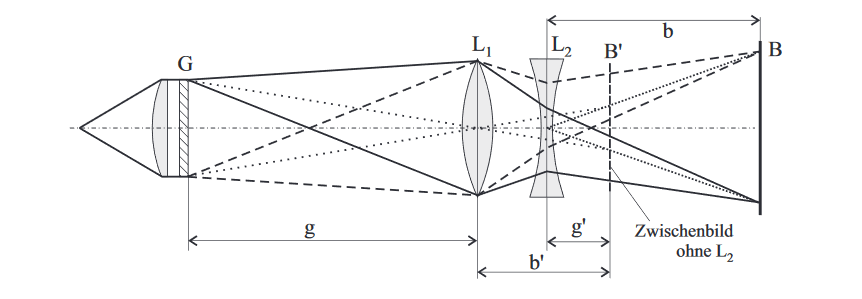
\includegraphics[scale=0.5]{zerstreuungslinse.png}
\caption{Kombination einer Sammelinse $L_1$ mit einer Zerstreuungslinse $L_2$. $G$ Gegenstand, $B^\prime$ Bild mit $L_1$ ohne $L_2$, $B$ Bild mit $L_1$ und $L_2$, $g$, $g^\prime$ Gegenstandsweite, $b$, $b^\prime$ Bildweite.}
\label{fig:zerstreuungslinse}
\end{figure}


\subsubsection{Methode 2}
Verändert man den Abstand der Zerstreuungslinse $L_2$ von $B^\prime$ derart, dass $g^\prime = -f_2$ wird, so rückt das Bild $B$ ins Unendliche, was mit einem auf \textit{Unendlich} justierten Fernrohr festgestellt werden kann, und eine direkte Brennweitenbestimmung leicht ermöglicht.

\newpage

\section{Geräteliste}

\begin{table}[H]
\caption{Liste der verwendeten Geräte}

~

\begin{tabular}{l|ll}
Bezeichnung & Inventarnummer & Unsicherheit \\
\hline
Sammellinse & V221 & \\
Zerstreuungslinse &  & \\
Lampe & V/747/4 & \\
Gegenstand & F4 & \\
Schirm & V/539/32 & \\
Maßband & & $\pm1~$mm
\end{tabular}

\end{table}




\section{Durchführung und Messwerte}

\subsection{Brennweite der Sammellinse nach Laplace}

Es werden 10 Messungen durchgeführt. Bei jeder Messung wird die Position die Gegenstands- und Bildweite, sowie die Position der Linse gemessen. Die Positionen werden relativ zu einem Fixpunkt gemessen. Die Messwerte sind in Tabelle \ref{tab:laplace_messung} dargestellt.

\begin{table}[H]
\caption{Messwerte der Methode nach Laplace. $G$ Gegenstandsposition, $B$ Bildposition, $L$ Linsenposition}
\label{tab:laplace_messung}
\centering
\begin{tabular}{c|rrr}
Nr. & $G$ / cm & $B$ / cm & $L$ / cm \\
\hline
1 & 160 & 15 & 136.2\\
2 & 160 & 20 & 135.7\\
3 & 160 & 25 & 135.2\\
4 & 160 & 30 & 134.5\\
5 & 160 & 35 & 134.9\\
6 & 160 & 40 & 134.0\\
7 & 160 & 45 & 133.9\\
8 & 160 & 50 & 133.6\\
9 & 160 & 55 & 132.9\\
10 & 160 & 60 & 131.9
\end{tabular}

\end{table}

\subsection{Brennweite der Sammellinse nach Bessel}

Hier wird bei gegebener Position von Gegenstand und Bild die Linse auf die Positionen $L_1$ und $L_2$ verschoben. Es wird für 5 Fälle gemessen.


\begin{table}[H]
\caption{Messwerte der Methode nach Bessel. $G$ Gegenstandsposition, $B$ Bildposition, $L_1$, $L_2$ Linsenpositionen}
\label{tab:bessel_messung}
\centering
\begin{tabular}{c|rrrr}
Nr. & $G$ / cm & $B$ / cm & $L_1$ / cm & $L_2$ / cm \\
\hline
1 & 161 & 15 & 44.7 & 136.6\\
2 & 161 & 20 & 39.6 & 136.6\\
3 & 161 & 30 & 53.3 & 136.0\\
4 & 161 & 40 & 66.0 & 135.4\\
5 & 161 & 50 & 76.8 & 134.4
\end{tabular}

\end{table}


\subsection{Brennweite der Zerstreuungslinse}



\begin{table}[H]
\caption{Messwerte für die Zerstreuungslinse. $G$ Gegenstandsposition, $B^\prime$ Bildposition nur für Sammellinse,  $B$ Bildposition, $L_1$ Position v. Sammellinse, $L_2$ Positin von Zerstreuungslinse}
\label{tab:zerstreuungslinse_messung}
\centering
\begin{tabular}{c|rrrrr}
Nr. & $G$ / cm & $B^\prime$ / cm & $B$ / cm & $L_1$ / cm & $L_2$ / cm \\
\hline
1 & 161 & 80.2 & 20 & 120.6 & 99.0\\
2 & 161 & 80.2 & 24 & 120.6 & 98.8\\
3 & 161 & 80.2 & 27 & 120.6 & 98.6\\
4 & 161 & 80.2 & 29 & 120.6 & 98.5\\
5 & 161 & 80.2 & 32 & 120.6 & 98.3\\
6 & 161 & 80.2 & 34 & 120.6 & 98.1\\
7 & 161 & 80.2 & 36 & 120.6 & 98.0\\
8 & 161 & 80.2 & 38 & 120.6 & 97.9\\
9 & 161 & 80.2 & 40 & 120.6 & 97.7\\
10 & 161 & 80.2 & 42 & 120.6 & 97.4
\end{tabular}

\end{table}




\section{Auswertung}



\subsection{Laplace}

Die Größtunsicherheitsmethode für die Brennweite nach Laplace aus Gleichung \eqref{eq:laplace} ergibt
\begin{align*}
\Delta f = \left|\frac{\partial f}{\partial g}\right| \cdot \Delta g +  \left|\frac{\partial f}{\partial b}\right| \cdot \Delta b  = \left(\frac1g + \frac1b\right)^{-2}\cdot \left(\frac{\Delta g}{g^2} + \frac{\Delta b}{b^2}\right)
\end{align*}

~ 

Mit diesen Erkentnissen wird die Tabelle \ref{tab:laplace_messung} ausgewertet.

\begin{table}[H]
\caption{Auswertung für die Laplace-Methode. $g = G-L$ Gegenstandsweite, $b = L-B$ Bildweite, $f$ berechnete Brennweite, $\Delta f$ Unsicherheit}
\label{tab:laplace_auswertung}
\centering
\begin{tabular}{c|rrrr}
Nr. & $g$ / cm & $b$ / cm & $f$ / cm & $\Delta f$ / cm \\
\hline
1 & 23.8 & 121.2 & 19.89 & 0.44\\
2 & 24.3 & 115.7 & 20.08 & 0.43\\
3 & 24.8 & 110.2 & 20.24 & 0.42\\
4 & 25.5 & 104.5 & 20.50 & 0.41\\
5 & 25.1 & 99.9 & 20.06 & 0.41\\
6 & 26.0 & 94.0 & 20.37 & 0.40\\
7 & 26.1 & 88.9 & 20.18 & 0.39\\
8 & 26.4 & 83.6 & 20.06 & 0.38\\
9 & 27.1 & 77.9 & 20.11 & 0.37\\
10 & 28.1 & 71.9 & 20.20 & 0.36
\end{tabular}

\end{table}



\subsection{Bessel}

Die Größtunsicherheitsmethode für die Brennweite nach Bessel aus Gleichung \eqref{eq:bessel} ergibt
\begin{align*}
\Delta f = \left|\frac{\partial f}{\partial a}\right| \cdot \Delta a +  \left|\frac{\partial f}{\partial e}\right| \cdot \Delta e  = \frac{1}{4\cdot a^2}\cdot \left[ \left(a^2+e^2\right)\cdot \Delta a + 2\cdot a\cdot e \cdot \Delta e\right]
\end{align*}


\begin{table}[H]
\caption{Auswertung für die Bessel-Methode. $a = G-B$ Gesamtabstand, $e = |L_1-L_2|$ Verschiebung der Linse, $f$ berechnete Brennweite, $\Delta f$ Unsicherheit}
\label{tab:bessel_auswertung}
\centering
\begin{tabular}{c|rrrr}
Nr. & $a$ / cm & $e$ / cm & $f$ / cm & $\Delta f$ / cm \\
\hline
1 & 146 & 91.9 & 22.04 & 0.01\\
2 & 141 & 97.0 & 18.57 & 0.01\\
3 & 131 & 82.7 & 19.7 & 0.01\\
4 & 121 & 69.4 & 20.3 & 0.01\\
5 & 111 & 57.6 & 20.28 & 0.01
\end{tabular}

\end{table}


\subsection{Zerstreuungslinse}

Die Brennweite berechnet sich in dem Fall analog zur Laplace Methode mit
\begin{align}
\frac1f = \frac{1}{g^\prime} + \frac1b
\end{align}


\begin{table}[H]
\caption{Auswertung für die Zerstreuungslinse. $g^\prime = B^\prime - L_2$, $b = L_2 -B$, $f$ berechnete Brennweite, $\Delta f$ Unsicherheit}
\label{tab:zerstreuungslinse_auswertung}
\centering
\begin{tabular}{c|rrrr}
Nr. & $g^\prime$ / cm & $b$ / cm & $f$ / cm & $\Delta f$ / cm \\
\hline
1 & -13 & 25 & -27.08 & 0.11\\
2 & -17.5 & 59.0 & -24.88 & 0.04\\
3 & -15 & 35.4 & -26.03 & 0.07\\
4 & -16 & 43 & -25.48 & 0.06\\
5 & -14 & 30.7 & -25.74 & 0.08\\
6 & -18 & 62 & -25.36 & 0.04\\
7 & -19 & 73.7 & -25.6 & 0.04\\
8 & -12 & 23 & -25.09 & 0.11\\
9 & -11 & 18.4 & -27.35 & 0.17\\
10 & -19 & 78.7 & -25.05 & 0.04
\end{tabular}

\end{table}




\section{Zusammenfassung und Diskussion}

Für die Brennweite nach der Laplace-Messung gilt durch Mittelung 
\begin{align*}
f = (20.17 \pm 0.4)~\text{cm}\\\end{align*}


Für die Brennweite nach der Bessel-Messung gilt durch Mittelung 
\begin{align*}
f = (20.18 \pm 0.01)~\text{cm}\\\end{align*}


Für die Zerstreuungslinse gilt durch Mittelung 
\begin{align*}
f = (24.89 \pm 0.04)~\text{cm}\\\end{align*}


Die Methoden nach Laplace und Bessel ergeben unter Berücksichtigung der Unsicherheit dasselbe Ergebnis. Bei der Messung der Zerstreuungslinse werden zwei Linsenpositionen gemessen, was den höheren Fehler erklärt.

Die angenommene Unsicherheit setzt sich zusammen aus der Unsicherheit des Maßbandes ($\pm$ 0.1~cm), mit dem der jeweilige Linsenabstand gemessen wurde und der Unsicherheit die entsteht, wenn man ein Objekt scharf stellt (Schärfebereich), welche mit $\pm$ 0.2~cm abgeschätzt wurde.
Unbedingt zu beachten ist auch, dass bei der Ermittlung der Brennweite nach Bessel der Gegenstand und der Schirm relativ weit voneinander zu platzieren sind, um sichergehen zu können, dass auch immer ein Abstand von 4 Mal der Brennweite eingehalten werden kann, da sonst das Bessel'sche Verfahren nicht wirksam wäre. 


\newpage 
\appendix
\section{Python Skript}



\definecolor{commentgreen}{RGB}{2,112,10}
\definecolor{eminence}{RGB}{108,48,130}
\definecolor{weborange}{RGB}{255,165,0}
\definecolor{frenchplum}{RGB}{129,20,83}

\lstdefinelanguage{python}{
    morekeywords={def, for, range, abs, return},
    otherkeywords={<-,->, |>, \%\{, \}, \{, \, (, )},
    sensitive=true,
    morecomment=[l]{\#},
    morecomment=[n]{/*}{*/},
    morecomment=[s][\color{purple}]{:}{\ },
    morestring=[s][\color{orange}]"",
    commentstyle=\color{commentgreen},
    keywordstyle=\color{eminence},
    stringstyle=\color{red},
	basicstyle=\ttfamily,
	breaklines,
	showstringspaces=false,
	frame=tb
}
\lstinputlisting[language=Python,captionpos=b, label=lst:test,caption={Laplace Auswertung}]{generate_numbers_laplace.py}

\lstinputlisting[language=Python,captionpos=b, label=lst:test,caption={Bessel Auswertung}]{generate_numbers_bessel.py}


\lstinputlisting[language=Python,captionpos=b, label=lst:test,caption={Zerstreuungslinse Auswertung}]{generate_numbers_zerstreuungslinse.py}




\end{document}